\documentclass{article}

\usepackage[tmargin=0.5in,bmargin=0.25in]{geometry}
\usepackage{amsmath, amssymb, amsthm}
\usepackage{enumitem}
\usepackage{multicol}
\usepackage{graphicx}

\graphicspath{{./}}

\title{\vspace{-4ex}Math 341 Project 1}
\author{Isaac Boaz}

\renewcommand{\arraystretch}{1.2}

\begin{document}

\maketitle

\section*{Probability Questions}

\begin{enumerate}
    \item Both roles rely heavily on data analysis, with the ability to crunch vast amounts of information to make informed decisions being a vital aspect of each. In the fast-paced world of Formula One racing, Computer Science majors can utilize their skills in programming and data analysis to process the mountains of data generated by a race. \\
          Another similarity between these roles is the need for algorithmic thinking. In Formula One racing, strategists must break down complex variables like tire wear, fuel consumption, and track conditions into manageable components to develop effective race strategies. Similarly, Computer Science majors use algorithmic thinking to break down complex problems into smaller, more manageable pieces.
    \item As binomial only checks two outcomes (success or failure), we can assign a safety car leading as a success and otherwise as a failure. One thing to note is that these laps aren't necessarily independent, as each lap may have an impact on the safety car's deployments further down the line.
    \item The Poisson distribution measures the \# of occurrences of an event within a fixed time/space. A requirement of this distribution is that \(n \rightarrow \infty,\ p \rightarrow 0,\ \lambda = np\). As \(n\) represents the number of laps, we can assume that it should be relatively high (given a timespan of a few seasons for example). Similarly, we can assume the safety car's deployment rate should be relatively low.
    \item The \# of safety car deployments can be modeled as a Poisson distribution, and thus, the interval between each deployment can be represented by an exponential distribution.
    \item We can assume that the two time periods are independent of each other as they are disjoint.
    \item
          \begin{align*}
              P(X \geq t_1 + t_2 \mid X \geq t_1) & = P(X \geq t_2), t_1 \geq 0, t_2 \geq 0 \\
              t_1                                 & = 3                                     \\
              t_2                                 & = 5                                     \\
              P(X \geq 3 + 5 \mid X \geq 3)       & = P(X \geq 8 \mid X \geq 3)             \\
                                                  & = P(X \geq 5)
          \end{align*}

          As the memoryless' property name implies, the probability of an event occurring at a time \(t\) is independent of the time that has passed since the event occurred. Thus, the probability of an event occurring at time \(t_1 + t_2\) is independent of the probability of the event occurring at time \(t_1\). Therefore, the probability of an event occurring at time \(t_1 + t_2\) (given \(t_1\) has passed) is equal to the probability of the event occurring at time \(t_2\).
\end{enumerate}

\pagebreak

\section*{Statistics Questions}
\begin{enumerate}
    \item Judging by the best Poisson line fit, the distributions seem to follow a Poisson distribution.
    \item Since the Poisson distribution's equation is \(P(X = k) = \frac{\lambda^k e^{-\lambda}}{k!}\), we can see that as \(\lambda\) increases, the probability of an event occurring increases. Since Poisson takes in the average amount of times an event occurs within a given timespan, it makes sense to use the mean \# of accidents for \(\lambda\).
    \item In general it seems that the interval between safety car deployments follows an exponential distribution.
    \item Since the exponential distribution's equation is \(P(X \leq t) = 1 - e^{-\lambda t}\), we can see that as \(\lambda\) increases, the probability of an event occurring increases. Since exponential takes in the average amount of time between events, it makes sense to use the mean interval between safety car deployments (ie the inverse of \# of deployments within a set timespan) for \(\lambda\).
    \item
          \setlength{\columnsep}{-5.5cm}
          \begin{multicols}{2}
              \begin{tabular}{lr|}
                  \multicolumn{2}{c}{Means} \\
                  first\_half  & 0.7291667  \\
                  interval1    & 1.328827   \\
                  second\_half & 0.6960784  \\
                  interval2    & 1.421543
              \end{tabular}
              \\ \\
              Going by the given means, we can see that each interval is approximately the inverse of the \# of safety car deployments per half (i.e: interval \(\approx \frac{1}{\# of deployments}\)). This makes sense as the exponential distribution (time between deployments) is the distribution of the time between events, and the Poisson distribution (number of deployments within a timespan), are inversely related.
          \end{multicols}
    \item This dataset is not necessarily independent; additionally, the inteval dataset is exponentially distributed, not normally.
    \item The equation we use to calculate a CI does not assume the dataset is normally distributed. Additionally, since the two event times are disjoin they can be considered independent according to the Poisson distribution.
    \item In order for us to test the null hypothesis, we are testing that the means of the two are equal, and will use the t test results to determine if there is evidence against it.
    \item t.test() results:\\
          Two Sample t-test

          data:  interval1 and interval2
          t = -0.39129, df = 139, p-value = 0.6962 \\
          alternative hypothesis: true difference in means is not equal to 0 \\
          95 percent confidence interval:
          -0.5612108  0.3757772 \\
          sample estimates:
          mean of x, mean of y /
          1.328827, 1.421543


          Welch Two Sample t-test

          data:  interval1 and interval2
          t = -0.39133, df = 139, p-value = 0.6962 \\
          alternative hypothesis: true difference in means is not equal to 0 \\
          95 percent confidence interval:
          -0.5611611  0.3757275 \\
          sample estimates:
          mean of x, mean of y /
          1.328827, 1.421543
    \item Based purely on the given intervals by the tests, both intervals encapsulate 0 (having negative and positive on either end). As such, there is no statistically significant change in the distribution between these two time periods. \addtocounter{enumi}{1}
    \item
          \setlength{\columnsep}{0.4cm}
          \begin{multicols}{2}
              Looking at the Q-Q plot, we can see that the first dataset follows the exponential distribution more closely than after the introduction of the VSC.
              \\
              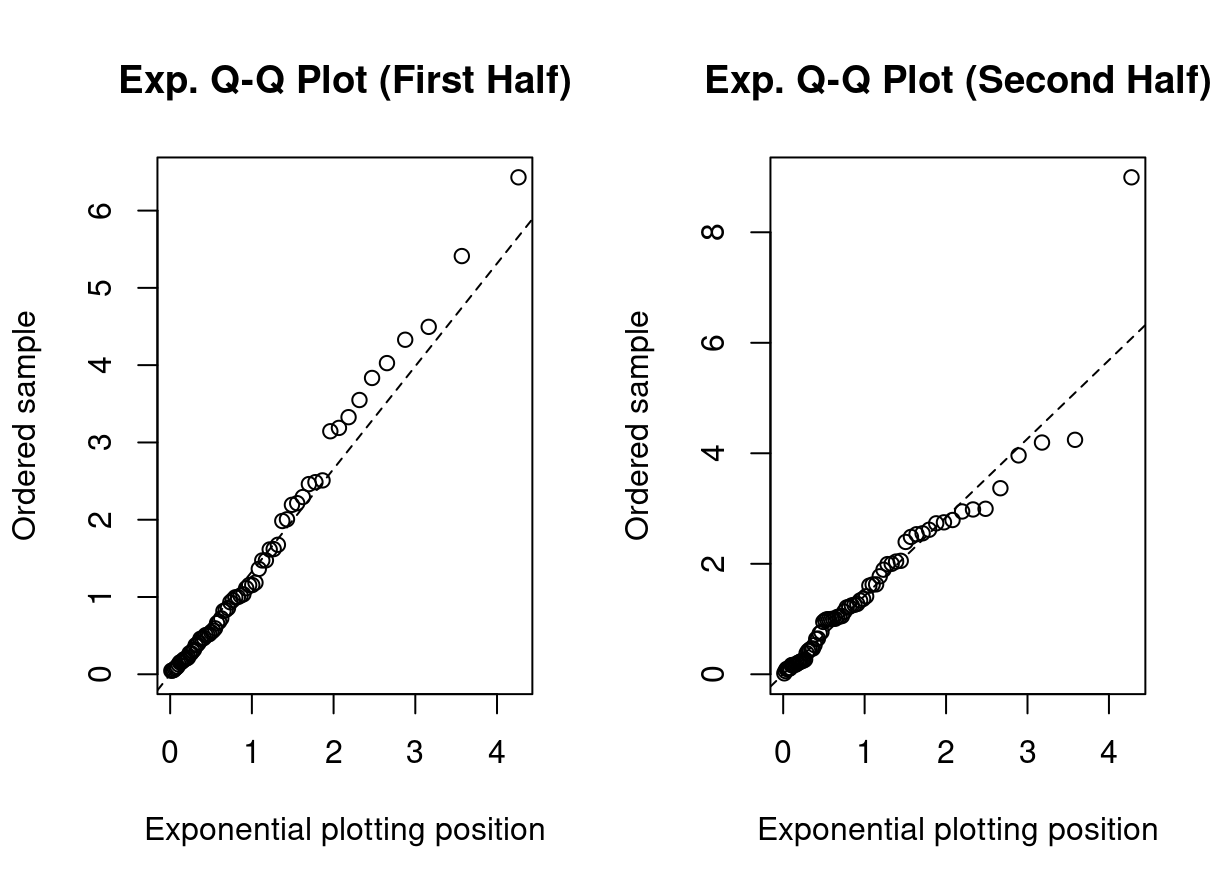
\includegraphics[scale=0.5]{q-qplot.png}
          \end{multicols}
    \item
          \begin{multicols}{2}
              The ACF plot shows us only one significant spike near the beginning of the dataset, which could be attributed to an outlier. Overall, there is a lack of evidence against independence. \\
              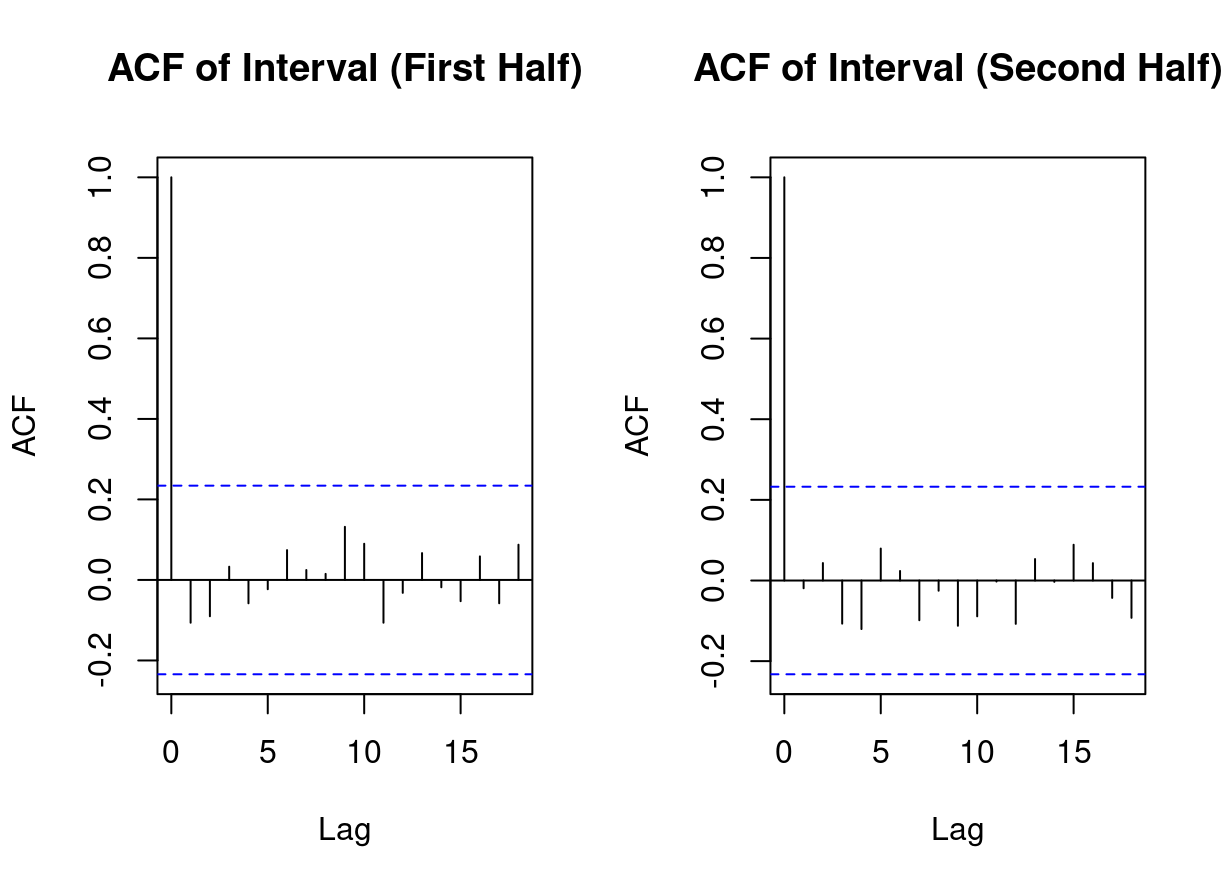
\includegraphics[scale=0.5]{acfplot.png}
          \end{multicols}
    \item This project introduced a lot of different statistical and probabilistic ideas. I think having a more thorough introduction of the formulas and equations covered (such as t tests) would more solidly introduce me to these ideas. Overall, this project taught me a lot about probability and statistics.
\end{enumerate}

\pagebreak
\section*{Team Description}
\begin{description}
    \item[Members] Isaac Boaz
    \item[Project Title] Formula One Racing Data Analysis
\end{description}

\end{document}